\documentclass[]{article}
\usepackage{amsmath}
\usepackage{amsfonts}
\usepackage{amssymb}
\usepackage{amsthm}
\usepackage{cancel}
\usepackage{graphicx}
\usepackage{pdfpages}
\usepackage{systeme}
\usepackage{hyperref}

\renewcommand{\thesection}{\arabic{section}}
\renewcommand{\thesubsection}{\thesection.\alph{subsection}}
\renewcommand{\thesubsubsection}{\thesubsection.\roman{subsubsection}}

\newtheorem{genthm}{Theorem}

\numberwithin{equation}{section}

%opening
\title{EECS 16A HW04}
\author{Bryan Ngo}
\date{2019-09-24}

\begin{document}

\maketitle

\section{Mechanical Inverses}

\subsection{}

\begin{align}
	&\left[
	\begin{array}{cc|cc}
	0 & 1 & 1 & 0 \\
	1 & 0 & 0 & 1
	\end{array}
	\right] \\
	\overset{r_1 \leftrightharpoons r_2}{\Longrightarrow} &\left[
	\begin{array}{cc|cc}
	1 & 0 & 0 & 1 \\
	0 & 1 & 1 & 0
	\end{array}
	\right] \\
	\mathbf{A}^{-1} &= 
	\begin{bmatrix}
	0 & 1 \\
	1 & 0
	\end{bmatrix}
\end{align}
\(\mathbf{A}\) reflects the vector across the line \(y = x\). 

\subsection{}

\begin{align}
	&\left[
	\begin{array}{cc|cc}
	-1 & 0 & 1 & 0 \\
	0 & 1 & 0 & 1
	\end{array}
	\right] \\
	\overset{-r_1 \to r_1}{\Longrightarrow} &\left[
	\begin{array}{cc|cc}
	1 & 0 & -1 & 0 \\
	0 & 1 & 0 & 1
	\end{array}
	\right] \\
	\mathbf{A}^{-1} &= 
	\begin{bmatrix}
	-1 & 0 \\
	0 & 1
	\end{bmatrix}
\end{align}
\(\mathbf{A}\) reflects the vector across the \(y\)-axis. 

\stepcounter{subsection}
\stepcounter{subsection}

\subsection{}

\begin{align}
	&\left[
	\begin{array}{cc|cc}
	1 & 1 & 1 & 0 \\
	2 & 0 & 0 & 1
	\end{array}
	\right] \\
	\overset{r_2 - 2r_1 \to r_2}{\Longrightarrow} &\left[
	\begin{array}{cc|cc}
	1 & 1 & 1 & 0 \\
	0 & -2 & -2 & 1
	\end{array}
	\right] \\
	\overset{r_2/-2 \to r_2}{\Longrightarrow} &\left[
	\begin{array}{cc|cc}
	1 & 1 & 1 & 0 \\
	0 & 1 & 1 & -\frac{1}{2}
	\end{array}
	\right] \\
	\overset{r_1 - r_2 \to r_1}{\Longrightarrow} &\left[
	\begin{array}{cc|cc}
	1 & 0 & 0 & \frac{1}{2} \\
	0 & 1 & 1 & -\frac{1}{2}
	\end{array}
	\right] \\
	\mathbf{A}^{-1} &= 
	\begin{bmatrix}
	0 & \frac{1}{2} \\
	1 & -\frac{1}{2}
	\end{bmatrix}
\end{align}
\(\mathbf{A}\) flips \(\hat{\jmath}\) to the \(x\)-axis and shears a given vector by 2. 

\subsection{}

\begin{align}
	&\left[
	\begin{array}{ccc|ccc}
	1 & 0 & 0 & 1 & 0 & 0 \\
	0 & 2 & 2 & 0 & 1 & 0 \\
	1 & 4 & 4 & 0 & 0 & 1
	\end{array}
	\right] \\
	\overset{r_3 - r_1 \to r_3}{\Longrightarrow} &\left[
	\begin{array}{ccc|ccc}
	1 & 0 & 0 & 1 & 0 & 0 \\
	0 & 2 & 2 & 0 & 1 & 0 \\
	0 & 4 & 4 & -1 & 0 & 1
	\end{array}
	\right] \\
	\overset{2r_2 \to r_2}{\Longrightarrow} &\left[
	\begin{array}{ccc|ccc}
	1 & 0 & 0 & 1 & 0 & 0 \\
	0 & 4 & 4 & 0 & 2 & 0 \\
	0 & 4 & 4 & -1 & 0 & 1
	\end{array}
	\right] \\
	\overset{r_3 - r_2 \to r_3}{\Longrightarrow} &\left[
	\begin{array}{ccc|ccc}
	1 & 0 & 0 & 1 & 0 & 0 \\
	0 & 4 & 4 & 0 & 2 & 0 \\
	0 & 0 & 0 & -1 & -2 & 1
	\end{array}
	\right]
\end{align}
The row of zeroes indicates that \(\mathbf{A}^{-1}\) does \emph{not} exist. \\
\\
\(\mathbf{A}\) flattens the \(x\)-component to the \(xz\)-plane, then flattens the \(y\)-component and \(z\)-component to the \(yz\)-plane. 

\section{Finding Null Spaces and Column Spaces}

\subsection{}

The maximum number of linearly independent columns in a \(3 \times 5\) matrix is 3, since there are 3 possible pivots in the matrix. 

\subsection{}

Given our matrix 
\begin{equation}
	\mathbf{A} = 
	\begin{bmatrix}
	1 & 1 & 0 & -2 & 3 \\
	0 & 0 & 1 & -1 & 1 \\
	0 & 0 & 0 & 0 & 0
	\end{bmatrix}
\end{equation}
\(\operatorname{colsp}(\mathbf{A}) \in \mathbb{R}^3\) even if there are all zeroes in the last row. Thus, we need only pick a basis set of vectors to satisfy the columnspace. Since the last two vectors can be made out of a linear combination of the 2nd and 3rd, they are within the span of the 2nd and 3rd columns. The choice is obvious that
\begin{gather}
	\operatorname{colsp}(\mathbf{A}) = \operatorname{span}\left\lbrace\begin{bmatrix}
	1 \\
	0 \\
	\end{bmatrix},\begin{bmatrix}
	0 \\
	1 \\
	\end{bmatrix}\right\rbrace = \mathbb{R}^2
\end{gather}
meaning the columnspace has dimension 2. 

\subsection{}

\begin{equation}
	\operatorname{null}(\mathbf{A}) = 
	\left[
	\begin{array}{ccccc|c}
	1 & 1 & 0 & -2 & 3  & 0 \\
	0 & 0 & 1 & -1 & 1 & 0 \\
	0 & 0 & 0 & 0 & 0 & 0
	\end{array}
	\right]
\end{equation}
The row of zeroes indicates that the nullspace is infinite. A system of linear equations of this matrix would look like
\begin{equation}
	\sysdelim..\systeme{x_1 + x_2 - 2x_4 + 3x_5 = 0, x_3 - x_4 + x_5 = 0, 0 = 0}
\end{equation}
Thus, we must express our nullspace in terms of our free variables, which in this case is \(x_{2,4,5}\) for the \(x_n\) column. This means we can express our nullspace as 
\begin{equation}
	\sysdelim..\systeme*{x_1 = -x_2 + 2x_4 - 3x_5, x_2 = x_2, x_3 = x_4 - x_5, x_4 = x_4, x_5 = x_5}
\end{equation}
Separating our free variables into vectors: 
\begin{align}
	\begin{bmatrix}
	x_1 \\
	x_2 \\
	x_3 \\
	x_4 \\
	x_5
	\end{bmatrix}
	&=
	\begin{bmatrix}
	-x_2 + 2x_4 - 3x_5 \\
	x_2 \\
	x_4 - x_5 \\
	x_4 \\
	x_5
	\end{bmatrix} \\
	&=
	\begin{bmatrix}
	-x_2 \\
	x_2 \\
	0 \\
	0 \\
	0
	\end{bmatrix} + 
	\begin{bmatrix}
	2x_4 \\
	0 \\
	x_4 \\
	x_4 \\
	0
	\end{bmatrix} + 
	\begin{bmatrix}
	-3x_5 \\
	0 \\
	-x_5 \\
	0 \\
	x_5
	\end{bmatrix} \\
	&=
	x_2 \begin{bmatrix}
	-1 \\
	1 \\
	0 \\
	0 \\
	0
	\end{bmatrix} + 
	x_4 \begin{bmatrix}
	2 \\
	0 \\
	1 \\
	1 \\
	0
	\end{bmatrix} + 
	x_5 \begin{bmatrix}
	-3 \\
	0 \\
	-1 \\
	0 \\
	1
	\end{bmatrix}
\end{align}
Since every vector in the nullspace can be written as a linear combination of the free variables, the three column vectors form a basis for the nullspace: 
\begin{equation}
	\operatorname{null}(\mathbf{A}) = \operatorname{span}\left\lbrace
	\begin{bmatrix}
	-1 \\
	1 \\
	0 \\
	0 \\
	0
	\end{bmatrix},
	\begin{bmatrix}
	2 \\
	0 \\
	1 \\
	1 \\
	0
	\end{bmatrix},
	\begin{bmatrix}
	-3 \\
	0 \\
	-1 \\
	0 \\
	1
	\end{bmatrix}
	\right\rbrace
\end{equation}
meaning the nullspace has dimension 3. 

\subsection{}

The sum of the dimensions of the nullspace and the columnspace is the number of columns in \(\mathbf{A}\). 

\stepcounter{subsection}
\stepcounter{subsection}

\section{Properties of Pump Systems}

\subsection{}

\begin{genthm}
	Consider a system consisting of two reservoirs such that the entries of each column in the system’s state transition matrix sum to one. If \(s\) is the total amount of water in the system at timestep \(n\), then the total amount of water at timestep \(n + 1\) will also be \(s\).
\end{genthm}

\subsection{}

We are given two reservoirs, meaning that the system can be written as a matrix-vector multiplication
\begin{equation}
	\underbrace{\begin{bmatrix}
	x_1[n + 1] \\
	x_2[n + 1]
	\end{bmatrix}}_{\mathbf{x}[n + 1]}
	= 
	\underbrace{\begin{bmatrix}
	a_{11} & a_{12} \\
	a_{21} & a_{22}
	\end{bmatrix}}_{\mathbf{A}}
	\underbrace{\begin{bmatrix}
	x_1[n] \\
	x_2[n]
	\end{bmatrix}}_{\mathbf{x}[n]}
\end{equation}
where we are given the constraint that 
\begin{equation}
	a_{11} + a_{21} = a_{12} + a_{22} = 1
\end{equation}

\subsection{}

What we are trying to prove is that
\begin{equation}\label{eq:3-c}
	s_3 + s_4 = s_1 + s_2
\end{equation}
under the transformation
\begin{equation}
	\begin{bmatrix}
	s_3 \\
	s_4
	\end{bmatrix}
	=
	\mathbf{A} \begin{bmatrix}
	s_1 \\
	s_2
	\end{bmatrix}
\end{equation}
for some state vector \(\mathbf{s}\). 

\subsection{}

\begin{proof}
Given our matrix multiplication
\begin{equation}
	\begin{bmatrix}
	s_3 \\
	s_4
	\end{bmatrix}
	=
	\begin{bmatrix}
	a_{11} & a_{12} \\
	a_{21} & a_{22}
	\end{bmatrix}
	\begin{bmatrix}
	s_1 \\
	s_2
	\end{bmatrix}
\end{equation}
If we carry out the matrix multiplication,
\begin{align}
	\begin{bmatrix}
	s_3 \\
	s_4
	\end{bmatrix}
	&=
	s_1 \begin{bmatrix}
	a_{11} \\
	a_{21}
	\end{bmatrix} + 
	s_2 \begin{bmatrix}
	a_{12} \\
	a_{22}
	\end{bmatrix} \\
	&= 
	\begin{bmatrix}
	s_1 a_{11} + s_2 a_{12} \\
	s_1 a_{21} + s_2 a_{22}
	\end{bmatrix}
\end{align}
Suppose we take the sum of \(s_{3,4}\). If we rearrange the terms and factor out \(s_{1,2}\),
\begin{align}
	s_3 + s_4 &= s_1 a_{11} + s_2 a_{12} + s_1 a_{21} + s_2 a_{22} \\
	&= s_1 (\cancelto{1}{a_{11} + a_{21}}) + s_2 (\cancelto{1}{a_{12} + a_{22}}) \\
	&= s_1 + s_2
\end{align}
\end{proof}

\subsection{}

\begin{genthm}
Given the matrix-vector multiplication
\begin{equation}
	\underbrace{\begin{bmatrix}
	x_1[n + 1] \\
	x_2[n + 1] \\
	\vdots \\
	x_k[n + 1]
	\end{bmatrix}}_{\mathbf{x}[n + 1]}
	= 
	\underbrace{\begin{bmatrix}
	a_{11} & a_{12} & \cdots & a_{1k} \\
	a_{21} & a_{22} & \cdots & a_{2k} \\
	\vdots & \vdots & \ddots & \vdots \\
	a_{m1} & a_{m2} & \cdots & a_{mk}
	\end{bmatrix}}_{\mathbf{A}}
	\underbrace{\begin{bmatrix}
	x_1[n] \\
	x_2[n] \\
	\vdots \\
	x_k[n]
	\end{bmatrix}}_{\mathbf{x}[n]}
\end{equation}
for some state vector \(\mathbf{x}[n]\) with \(k\) unknowns multiplied by a transition matrix \(\mathbf{A} \in \mathbb{R}^{m \times k}\), where
\begin{equation}\label{eq:3-e}
	\sum_{i = 1}^{m} a_{i1} = \sum_{i = 1}^{m} a_{i2} = \cdots = \sum_{i = 1}^{m} a_{ik} = 1
\end{equation}
then it follows that 
\begin{equation}
	\sum_{i = 1}^{k} x_i[n + 1] = \sum_{i = 1}^{k} x_i[n]
\end{equation}
\end{genthm}

\begin{proof}
Carrying out the matrix multiplication,
\begin{align}
	\begin{bmatrix}
	x_1[n + 1] \\
	x_2[n + 1] \\
	\vdots \\
	x_k[n + 1]
	\end{bmatrix}
	&= x_1[n] \begin{bmatrix}
	a_{11} \\
	a_{21} \\
	\vdots \\
	a_{m1}
	\end{bmatrix} + 
	x_2[n] \begin{bmatrix}
	a_{12} \\
	a_{22} \\
	\vdots \\
	a_{m2}
	\end{bmatrix} + \cdots + 
	x_k[n] \begin{bmatrix}
	a_{1k} \\
	a_{2k} \\
	\vdots \\
	a_{mk}
	\end{bmatrix} \\
	&= \begin{bmatrix}
	x_1[n] a_{11} + x_2[n] a_{12} + \cdots + x_k[n] a_{1k} \\
	x_1[n] a_{21} + x_2[n] a_{22} + \cdots + x_k[n] a_{2k} \\
	\vdots \\
	x_1[n] a_{m1} + x_2[n] a_{m2} + \cdots + x_k[n] a_{mk}
	\end{bmatrix}
\end{align}
Suppose we take the sum of the entries of \(\mathbf{x}[n + 1]\), We can rearrange the sum such that we can factor out the components of the state vector. Then using the given information in \autoref{eq:3-e}, we can cancel those sums to 1: 
\begin{gather}
	\sum_{i = 1}^{k} x_i[n + 1] = x_1[n] (\cancelto{1}{a_{11} + a_{21} + \cdots + a_{m1}}) + x_2[n] (\cancelto{1}{a_{12} + a_{22} + \cdots + a_{m2}}) + \cdots \\
	\sum_{i = 1}^{k} x_i[n + 1] = \sum_{i = 1}^{k} x_k[n]
\end{gather}
\end{proof}

\stepcounter{subsection}
\stepcounter{subsection}
\stepcounter{subsection}
\stepcounter{subsection}
\stepcounter{subsection}

\section{Traffic Flows}

\subsection{}

Given \(t_1\), we can determine the values of \(t_{2,3}\). This is because \(t_{2,3}\) is defined in terms of \(t_1\). In the example given, we have
\begin{equation}
	\sysdelim..\systeme{10 + t_3 = 0, t_2 - 10 = 0}
\end{equation}
meaning that 
\begin{equation}
	\begin{array}{c}
	t_1 = 10 \\
	t_2 = 10 \\
	t_3 = -10
	\end{array}
\end{equation}

\subsection{}

We can represent the given diagram as 
\begin{equation}\label{eq:4-b}
	\sysdelim..\systeme{t_1 + t_3 - t_4 = 0, -t_1 + t_2 = 0, -t_2 - t_3 + t_5 = 0, t_4 - t_5 = 0}
\end{equation}
If we know \(t_{3,5}\) according to the Berkeley student, then it is possible to deduce the rest of the traffic vector, by first determining \(t_{2,4}\), then using it to determine \(t_1\). On the other hand, knowing \(t_{1,2}\) renders it impossible to determine the rest of the traffic vector because there is no way to recover any of the other vectors. This means the Berkeley student's sensor placement is superior.\footnote{Go Bears!}

\subsection{}

Given \autoref{eq:4-b}, we can construct a transition matrix out of the road system
\begin{equation}
	\underbrace{\begin{bmatrix}
	1 & 0 & 1 & -1 & 0 \\
	-1 & 1 & 0 & 0 & 0 \\
	0 & -1 & -1 & 0 & 1 \\
	0 & 0 & 0 & 1 & -1
	\end{bmatrix}}_{\mathbf{B}}
	\begin{bmatrix}
	t_1 \\
	t_2 \\
	t_3 \\
	t_4 \\
	t_5
	\end{bmatrix}
	= 
	\begin{bmatrix}
	0 \\
	0 \\
	0 \\
	0 \\
	0
	\end{bmatrix}
\end{equation}
The sum of the columns of \(\mathbf{B}\) is 0, representing the fact that the net flux of traffic is zero. 

\subsection{}

Finding the nullspace of \(\mathbf{B}\), 
\begin{align}
	\operatorname{null}(\mathbf{B}) = 
	&\left[
	\begin{array}{ccccc|c}
	1 & 0 & 1 & -1 & 0 & 0 \\
	-1 & 1 & 0 & 0 & 0 & 0 \\
	0 & -1 & -1 & 0 & 1 & 0 \\
	0 & 0 & 0 & 1 & -1 & 0
	\end{array}
	\right] \\
	\overset{r_2 + r_1 \to r_2}{\Longrightarrow} &\left[
	\begin{array}{ccccc|c}
	1 & 0 & 1 & -1 & 0 & 0 \\
	0 & 1 & 1 & -1 & 0 & 0 \\
	0 & -1 & -1 & 0 & 1 & 0 \\
	0 & 0 & 0 & 1 & -1 & 0
	\end{array}
	\right] \\
	\overset{r_3 + r_2 \to b_3}{\Longrightarrow} &\left[
	\begin{array}{ccccc|c}
	1 & 0 & 1 & -1 & 0 & 0 \\
	0 & 1 & 1 & -1 & 0 & 0 \\
	0 & 0 & 0 & -1 & 1 & 0 \\
	0 & 0 & 0 & 1 & -1 & 0
	\end{array}
	\right] \\
	\overset{-r_4 \to r_4}{\Longrightarrow} &\left[
	\begin{array}{ccccc|c}
	1 & 0 & 1 & -1 & 0 & 0 \\
	0 & 1 & 1 & -1 & 0 & 0 \\
	0 & 0 & 0 & 1 & -1 & 0 \\
	0 & 0 & 0 & 1 & -1 & 0
	\end{array}
	\right] \\
	\overset{r_4 + r_3 \to r_4}{\Longrightarrow} &\left[
	\begin{array}{ccccc|c}
	1 & 0 & 1 & -1 & 0 & 0 \\
	0 & 1 & 1 & -1 & 0 & 0 \\
	0 & 0 & 0 & 1 & -1 & 0 \\
	0 & 0 & 0 & 0 & 0 & 0
	\end{array}
	\right] \\
	\overset{r_3 + r_4 \to r_3}{\Longrightarrow} &\left[
	\begin{array}{ccccc|c}
	1 & 0 & 1 & -1 & 0 & 0 \\
	0 & 1 & 1 & 0 & -1 & 0 \\
	0 & 0 & 0 & 1 & -1 & 0 \\
	0 & 0 & 0 & 0 & 0 & 0
	\end{array}
	\right] \\
	\overset{r_2 + r_4 \to r_2}{\Longrightarrow} &\left[
	\begin{array}{ccccc|c}
	1 & 0 & 1 & 0 & -1 & 0 \\
	0 & 1 & 1 & 0 & -1 & 0 \\
	0 & 0 & 0 & 1 & -1 & 0 \\
	0 & 0 & 0 & 0 & 0 & 0
	\end{array}
	\right]
\end{align}
We end up with a row of zeroes, meaning that our nullspace can be represented as a linear combination of basis vectors. Our free variables are \(t_{3,5}\). Solving for the vectors in terms of the free variables and reconverting to a system of linear equations: 
\begin{align}
	\begin{bmatrix}
	x_1 \\
	x_2 \\
	x_3 \\
	x_4 \\
	x_5
	\end{bmatrix}
	&= 
	\begin{bmatrix}
	-x_3 + x_5 \\
	-x_3 + x_5 \\
	x_3 \\
	x_5 \\
	x_5
	\end{bmatrix} \\
	&= 
	x_3 \begin{bmatrix}
	-1 \\
	-1 \\
	1 \\
	0 \\
	0
	\end{bmatrix} + 
	x_5 \begin{bmatrix}
	1 \\
	1 \\
	0 \\
	1 \\
	1
	\end{bmatrix}
\end{align}
meaning our nullspace is 
\begin{equation}
	\operatorname{null}(\mathbf{B}) = \operatorname{span}\left\lbrace
	\begin{bmatrix}
	-1 \\
	-1 \\
	1 \\
	0 \\
	0
	\end{bmatrix}, 
	\begin{bmatrix}
	1 \\
	1 \\
	0 \\
	1 \\
	1
	\end{bmatrix}
	\right\rbrace
\end{equation}
The dimension of the nullspace is 2. 

\subsection{}

The Stanford measurement is 
\begin{equation}
	\mathbf{M}_{S} \mathbf{t} = \begin{bmatrix}
	1 & 0 & 0 & 0 & 0 \\
	0 & 1 & 0 & 0 & 0
	\end{bmatrix} \mathbf{t}
	=
	\begin{bmatrix}
	t_1 \\
	t_2
	\end{bmatrix}
\end{equation}

\subsection{}

The statement is not true, given the Stanford vector as a counterexample. Even though the dimension of the nullspace was 2, 2 measurements was not sufficient to resolve the system. 

\section{Segway Tours}

\subsection{}

\begin{equation}
	\mathbf{x}[1] = \mathbf{Ax}[0] + \mathbf{b}u[0]
\end{equation}

\subsection{}

\begin{align}
	\mathbf{x}[2] &= \mathbf{A}^2 \mathbf{x}[0] + \mathbf{Ab} u[0] + \mathbf{b} u[1] \\
	\mathbf{x}[3] &= \mathbf{A}^3 \mathbf{x}[0] + \mathbf{A}^2 \mathbf{b} u[0] + \mathbf{A} \mathbf{b} u[1] + \mathbf{b} u[2] \\
	\mathbf{x}[4] &= \mathbf{A}^4 \mathbf{x}[0] + \mathbf{A}^3 \mathbf{b} u[0] + \mathbf{A}^2 \mathbf{b} u[1] + \mathbf{A} \mathbf{b} u[2] + \mathbf{b} u[3]
\end{align}

\subsection{}

\begin{equation}
	\mathbf{x}[N] = \sum_{i = 1}^{N} \mathbf{A}^i \mathbf{x}[0] + \sum_{i = 0}^{N - 1} \mathbf{A}^{N - 1 - i} \mathbf{b} u[i]
\end{equation}

\subsection{}

Isolating the scalars and converting to a matrix-vector multiplication, 
\begin{align}
	\cancelto{0}{\mathbf{x}[2]} - \mathbf{A}^2 \mathbf{x}[0] &= \mathbf{Ab} u[0] + \mathbf{b} u[1] \\
	-\mathbf{A}^2 \mathbf{x}[0] &= 
	\begin{bmatrix}
	\mathbf{Ab} & \mathbf{b}
	\end{bmatrix}
	\begin{bmatrix}
	u[0] \\
	u[1]
	\end{bmatrix}\label{eq:5-d}
\end{align}
When Gaussian elimination is performed on \(\begin{bmatrix}
\mathbf{Ab} & \mathbf{b}
\end{bmatrix}\), the \texttt{iPython} notebook returns the matrix
\begin{equation}
	\begin{bmatrix}
	1 & 0 \\
	0 & 1 \\
	0 & 0 \\
	0 & 0
	\end{bmatrix}
\end{equation}
the row of zeroes indicates that it is impossible to find a solution with only two timesteps. 

\subsection{}

Plugging in the following matrix 
\begin{equation}
	-\mathbf{A}^3 x[0] = 
	\begin{bmatrix}
	\mathbf{A}^2 \mathbf{b} & \mathbf{Ab} & \mathbf{b}
	\end{bmatrix}
	\begin{bmatrix}
	u[0] \\
	u[1] \\
	u[2]
	\end{bmatrix}
\end{equation}
We get our reduced matrix
\begin{equation}
	\begin{bmatrix}
	1 & 0 & 0 \\
	0 & 1 & 0 \\
	0 & 0 & 1 \\
	0 & 0 & 0
	\end{bmatrix}
\end{equation}
Once more indicating it is impossible to find the unique control solution with three timesteps. 

\subsection{}

Plugging in the following matrix 
\begin{equation}
	-\mathbf{A}^4 x[0] = 
	\begin{bmatrix}
	\mathbf{A}^3 \mathbf{b} & \mathbf{A}^2 \mathbf{b} & \mathbf{Ab} & \mathbf{b}
	\end{bmatrix}
	\begin{bmatrix}
	u[0] \\
	u[1] \\
	u[2] \\
	u[3]
	\end{bmatrix}
\end{equation}
We get our reduced matrix
\begin{equation}
	\begin{bmatrix}
		1 & 0 & 0 & 0 \\
		0 & 1 & 0 & 0 \\
		0 & 0 & 1 & 0 \\
		0 & 0 & 0 & 1
	\end{bmatrix}
\end{equation}
meaning that a unique solution is possible with four timesteps. 

\subsection{}

See \texttt{iPython} notebook. 

\subsection{}

The vectors we are allowed to move in in two timesteps is \(\mathbf{Ab}, \mathbf{b}\). It follows that the range of possible controls within two timesteps is \(\operatorname{span}\{\mathbf{Ab},
\mathbf{b}\}\). 

\subsection{}

We can generalize this to say that the possible controls for any \(N\) timesteps is 
\begin{equation}
	\operatorname{colsp}(\begin{bmatrix}
	A^{N - 1} \mathbf{b} & \mathbf{A}^{N - 2} \mathbf{b} & \cdots & \mathbf{b}
	\end{bmatrix}) = \operatorname{span}\{A^{N - 1} \mathbf{b}, \mathbf{A}^{N - 2} \mathbf{b}, \ldots, \mathbf{b}\}
\end{equation}

\stepcounter{subsection}

\stepcounter{section}

\section{Homework Process and Study Group}

I worked on this homework by myself. 

\newpage

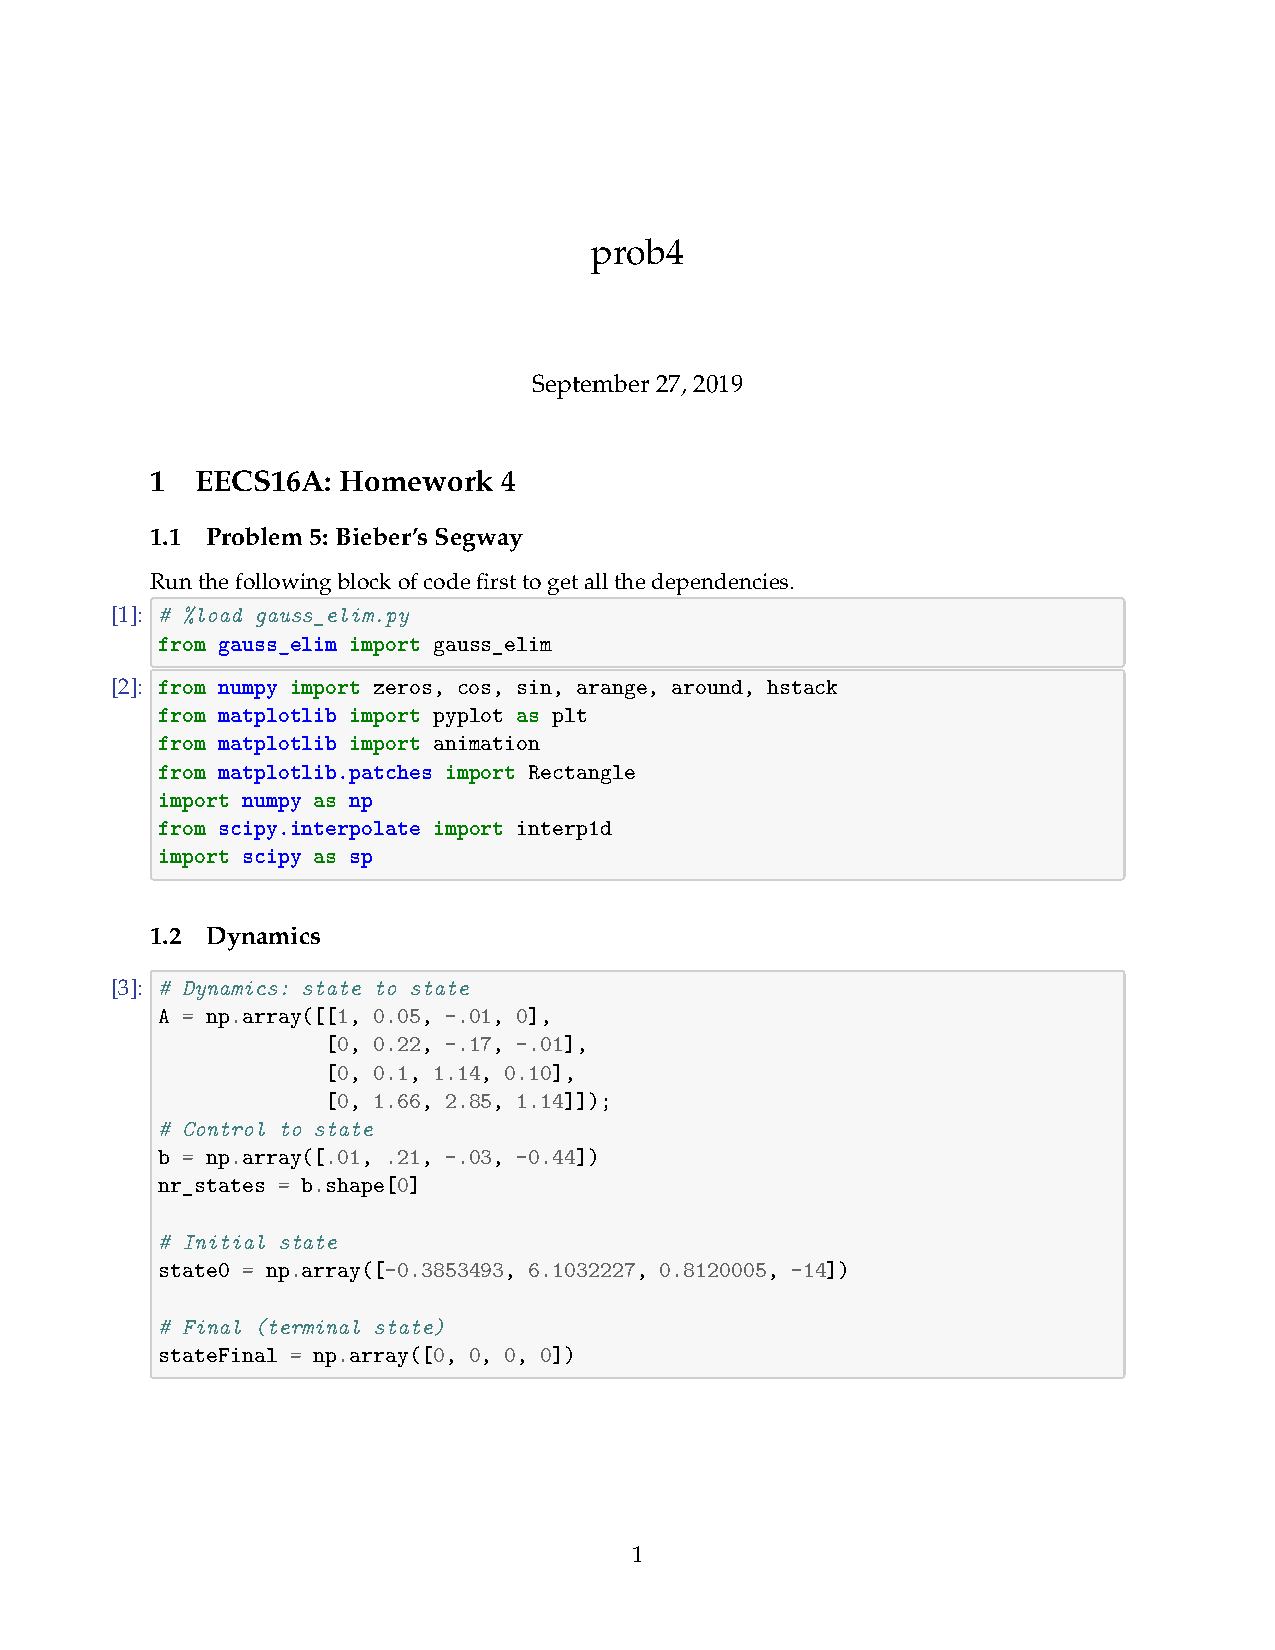
\includepdf[pages=-]{prob4.pdf}

\end{document}